\section{Separation von Amplitude und Phase}
\label{complex:separate}
\rhead{Separation Amplitude / Phase}
\subsection{Warum komplex?}
Das Problem der Separation von Betrag und Winkel kennt man aus der Fourierteorie mit Cosinus und Sinus.
Die Variablen $a$ in der Wavelet-Transformation und $\omega$ bei Fourier erfüllen ähnliche Zwecke, die Verschiebung durch $b$ macht für unendlich lange Basisfunktionen aber nur bedingt Sinn.
Deshalb kommen bei Fourier nur zwei Familien an Basisfunktionen zum Einsatz, der Cosinus und die um 90\textdegree{} verschobene, orthogonale Version, der Sinus.
Im Abschnitt~\ref{subsection:complex-fourier-series} haben wir gesehen, wie man Fourierreihen mit komplexen Exponentialfunktionen berechnet.

Sinus und Cosinus liefern -- in Analogie zu einem Kreis -- kartesischen Koordinaten. 
Für eine Darstellung als Betrag und Winkel sind sie ungeeignet.
Die Basisfunktion
\begin{align*}
	z(t) = Ce^{i\omega t} &= |C|e^{i\left(\omega t + \arg C\right)}
\end{align*}
erlaubt hingegen durch 
\begin{align*}
	|z(t)| = |C| \quad \text{und}\quad
	\arg z = \arg \omega t + \arg C
\end{align*}
direkt eine separate Betrachtung von Amplitude und Winkel.

Komplexe Basisfunktionen alleine garantieren die Separierbarkeit von Betrag und Winkel jedoch noch nicht.
Jedes reelle Wavelet kann durch
\begin{align*}
	\mathbb{R} \hookrightarrow \mathbb{C} \colon \quad x \mapsto ix.
\end{align*}
als komplexes Wavelet aufgefasst werden.
Ausser einem zusätzlichen Faktor $i$ ist jedoch nichts pasiert.
Welche Anforderungen müssen also erfüllt sein, damit Betrag und Winkel wirklich voneinander unabhängig sind?

Aufgrund der eulerschen Formel
\begin{equation}
	\frac{e^{i\omega t} + e^{-i\omega t}}{2} = \cos(\omega t)\label{complex:euler}
\end{equation}
kann der Cosinus aus zwei komplexen Exponentialfunktionen mit inverser Frequenz dargestellt werden.
Negative Frequenzen führen also zu einem Problem.
Dies gilt auch, wenn die Amplituden der beiden Exponentialfunktionen nicht übereinstimmen, die Anwesenheit der negativen Frequenz reicht aus, damit ein Teil der Amplitude nicht von der Phase getrennt werden kann.
\begin{align*}
	\frac{e^{i\omega t} + \Delta e^{-i\omega t}}{2} &=
	\Delta\cos(\omega t) + \frac{1-\Delta}{2} e^{i\omega t}\\
\end{align*}
Ein solches $\Delta$ ``frisst'' uns quasi die erwünschte Exponentialfunktion davon.
Etwas ähnliches geschiet bei positiven, leich unterschiedlichen Frequenzen
\begin{align*}
	\frac{e^{i\omega_1 t} + e^{i\omega_2 t}}{2} &=
	\frac{e^{i(\overline\omega + \Delta \omega) t} + e^{i(\overline\omega-\Delta\omega) t}}{2} \\
	&= e^{i\overline\omega t}\cos(\Delta\omega t)
\end{align*}
Hierbei bezeichnet $\overline\omega=(\omega_1+\omega_2)/2$ die mittlere Frequenz und $\Delta\omega=(\omega_1-\omega_2)/2$ die mittlere Differenz.
Ein $\Delta\omega$ führt also zu einer an- und abschwellenden Exponentialfunktion.
Dies ist für Wavelets verkraftbar, da sie so wie so in der Zeit lokalisiert sind.
$\Delta\omega$ muss lediglich klein genug sein.

Daraus folgt, dass Amplitude und Phase nur dann separiert werden können, wenn die Fouriertransformierte des Wavelets für alle negativen Frequenzen verschwindet.
Besitzt ein Wavelet Frequenz-Anteile bei $\omega < 0$, dann geht bei diesen Frequenzen die Eigenschaft der Separierbarkeit von Amplitude und Phase verloren.

Fouriertransformierte von reellen Signalen weisen jedoch immer eine hermitesche Symmetrie auf, das heisst
\begin{align*}
	f(t)\in\mathbb R &\Rightarrow \hat f(\omega) = -\hat f(-\omega)
\end{align*}
Die einzigen, reellen Funktionen, deren Spektra für negative Frequenzen verschwindet, sind $f(t) = c$, $c\in\mathbb R$.
Eine solche Funktion erfüllt jedoch nicht die Bedingung $\|f\| = 1$.
Die reelle Mathematik stösst bei diesem Problem also an ihre Grenzen.

\subsection{Von Gabor zu Morlet}
\label{complex:gabor-to-morlet}
Durch die Cosinus-Funktion besitzt das Gabor-Wavelet negative Frequenzen.
Dies möchten wir im Folgenden korrigieren.
Wir wechseln in den Fourierbereich und nutzen aus, dass die Fouriertransformierte einer Gaus-Funktion wieder eine Gaus-Funktion ist,
\[
	\mathcal{F}\left\lbrace e^{-\alpha x^2} \right\rbrace 
	= \frac{1}{\sqrt{2\alpha}}e^{- \frac{\omega^2}{4\alpha}},
\]
und dass die Multiplikation im Zeitbereich zur Faltung im Frequenzbereich wird.
Zudem verwenden wir die Eulerformel~\eqref{complex:euler}.
Die Fouriertransformierte des Gabor-Wavelet wird hierdurch zu

\begin{equation*}
\begin{aligned}
 \hat{\psi}
 & = \mathcal{F}\Bigg\lbrace c_\sigma e^{-\frac{t^2}{2}}\phantom{\Bigg\rbrace}
 \cdot\; \phantom{\mathcal{F}\Bigg\lbrace}
 \Bigg(\cos\left(\sigma t\right) &&
 &&- \kappa_\sigma\Bigg) \Bigg\rbrace \\
 & = \mathcal{F}\Bigg\lbrace c_\sigma e^{-\frac{t^2}{2}} \Bigg\rbrace 
 *\: \mathcal{F}\Bigg\lbrace\Bigg( \frac12 e^{i\sigma t} &+& \frac12 e^{-i\sigma t}
 &&- \kappa_\sigma \Bigg)\Bigg\rbrace\\
 & = \phantom{\mathcal{F}\Bigg\lbrace} c_\sigma e^{- \frac{\omega^2}{2}} \phantom{\Big\rbrace}
 *\:\phantom{\mathcal{F}\Bigg\lbrace} \Bigg(
  \frac{1}{2}\delta(\omega - \sigma) &-&
  \frac{1}{2}\delta(\omega + \sigma) 
 && - \kappa_\sigma\delta(\omega)
  \Bigg).
\end{aligned}
\end{equation*}

Hierbei bezeichnet $\delta(\omega)$ die Dirac-Distribution.
Hieraus lässt sich der negative Anteil des Cosinus leicht entfernen.
Zudem verdoppeln wir den Anteil der positiven Frequenzen (der Grund hierfür erschliesst sich im nächsten Kapitel).
Wir erhalten
\[
	\hat{\psi}^\ast = 
	c_\sigma e^{- \frac{\omega^2}{2}} * \left(
	\delta(\omega - \sigma) +
	\kappa_\sigma\delta(\omega)
	\right),
\]
und durch Rücktransformation in den Zeitbereich
\[
	\psi^\ast = 
	c_\sigma e^{- \frac{t^2}{2}} \cdot \left(
	e^{i\sigma t} +
	\kappa_\sigma
	\right).
\]
Dies ist ein alter Bekannter, das Morlet-Wavelet aus Gleichung~\eqref{cwt:morlet}, dargestellt in Abbildung~\ref{complex:morlet}.
Es eignet sich also besonder gut, um bestimmte Frequenzen in einem Signal zu lokalisieren, allerdings ist es in der Zeit wesentlich schlechter lokalisiert als beispielsweise das Haar-Wavelet.
Dies ist auch in Abbildung~\ref{complex:morlet-ex} ersichtlich, welche die beiden Wavelet-Transformationen unserer Beispiel-Signale zeigt.

\begin{figure}
	\centering
	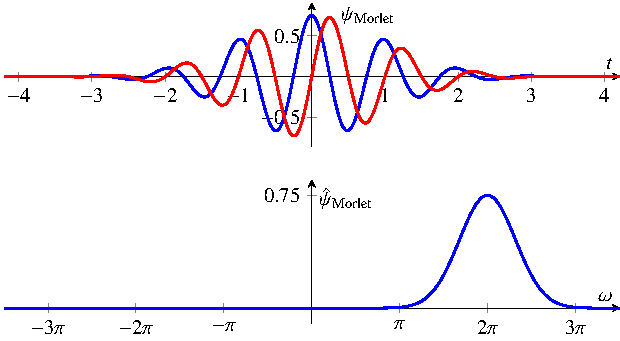
\includegraphics{papers/complex/images/morlet.pdf}
	\caption{Real- (blau) und Imaginärteil (rot) des Morlet-Wavelet für $\sigma = 2\pi$ \label{complex:morlet}}
\end{figure}

\begin{figure}
	\centering
	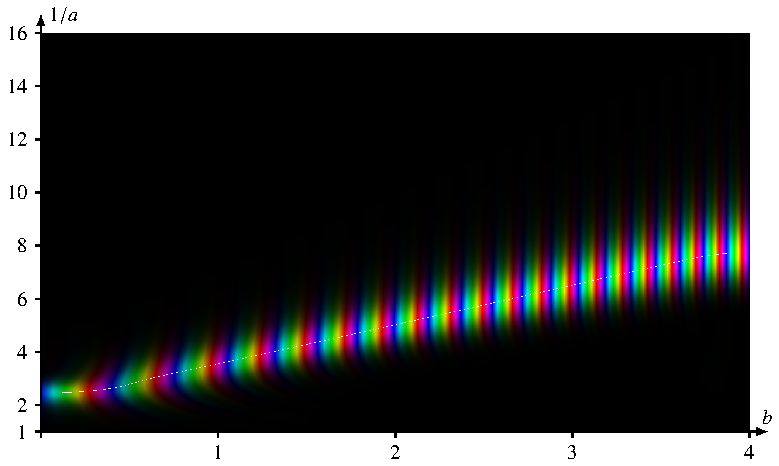
\includegraphics{papers/complex/images/chirp_morlet.pdf}
	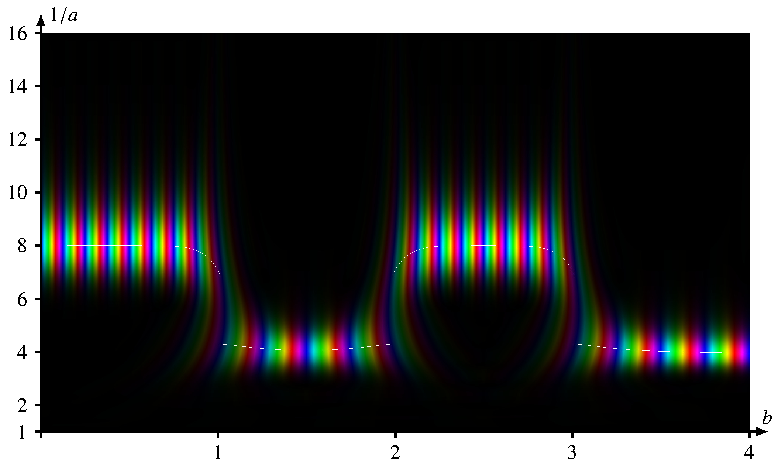
\includegraphics{papers/complex/images/square_morlet.pdf}
	\caption{Farb-codierte Wavelet-Transformationen der beiden Beispielsignale mit dem Morlet-Wavelet.}
	\label{complex:morlet-ex}
\end{figure}
